% This file contains text to create bios for EnICS members and close collaborators

%%%%%%%%%%%%%%%%%%%%%%%%%%%%%%%%%%%%%%%%%%%%%%%%%%%%
%%%                  Faculty                     %%%
%%%%%%%%%%%%%%%%%%%%%%%%%%%%%%%%%%%%%%%%%%%%%%%%%%%%

%<*AdamTeman>
\begin{IEEEbiography}    [{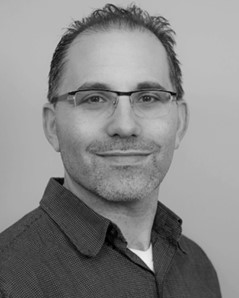
\includegraphics[width=1in,height=1.25in,clip,keepaspectratio]{./Bios/adam_teman.jpg}}]
    {Adam Teman} (Member, IEEE) received the Ph.D. degree in electrical and computer engineering from Ben-Gurion University (BGU), Be’er Sheva, in 2014. He worked as a Design Engineer at Marvell Semiconductors, from 2006 to 2007. From 2014 to 2015, he was a Postdoctoral Researcher at the École Polytechnique Fédérale de Lausanne (EPFL), Switzerland, under a Swiss Government Excellence Scholarship. Since 2015, he has been with Bar-Ilan University, where he is an Associate Professor and the Co-Director of the Emerging Nanoscaled Integrated Circuits and Systems (EnICS) Laboratories. In 2021, he co-founded RAAAM Memory Technologies, where he is head of Product Development. He has authored over 115 scientific articles and holds 11 patents. His research interests include embedded memories, energy-efficient circuit design, hardware for artificial intelligence, open source processor platforms and accelerators, and methodologies for physical implementation. In 2020, he was awarded the Krill Prize for outstanding young researchers. 
\end{IEEEbiography}
%</AdamTeman>

%<*LeonidYavits>
\begin{IEEEbiography}[{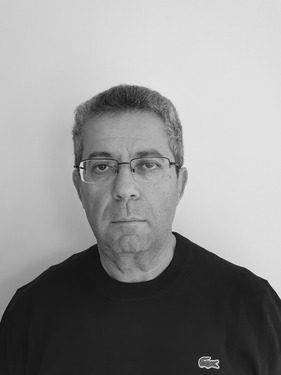
\includegraphics[angle=0,width=1in,height=1.25in,clip,keepaspectratio]{./Bios/leonid_yavits.jpg}}]{Leonid Yavits} 
    is with the Faculty of Engineering, Bar-Ilan University, Israel. He received his MSc and PhD degrees in electrical engineering from Technion, Israel. Leonid is a serial entrepreneur who was involved in co-founding and successful management (from a concept to M\&A) of several start-ups in the field of ASICs. His research interests include bioinformatics, domain specific accelerators, and processing in memory.
\end{IEEEbiography}
%</LeonidYavits>

%<*AlexFish>
\begin{IEEEbiography}    [{\includegraphics[width=1in,height=1.25in,clip,keepaspectratio]{./Bios/alex_fish.jpg}}]
    {Alex Fish} (Member, IEEE) . 
\end{IEEEbiography}
%</AlexFish>

%<*YossieShor>
\begin{IEEEbiography}    [{\includegraphics[width=1in,height=1.25in,clip,keepaspectratio]{./Bios/yossie_shor.jpg}}]
    {Yossie Shor} (Senior Member, IEEE) . 
\end{IEEEbiography}
%</YossieShor>

%<*ItamarLevy>
\begin{IEEEbiography}    [{\includegraphics[width=1in,height=1.25in,clip,keepaspectratio]{./Bios/itamar_levy.jpg}}]
    {Itamar Levy} (Member, IEEE) . 
\end{IEEEbiography}
%</ItamarLevy>

%<*OsnatKeren>
\begin{IEEEbiography}    [{\includegraphics[width=1in,height=1.25in,clip,keepaspectratio]{./Bios/osnat_keren.jpg}}]
    {Osnat Keren} (Member, IEEE) . 
\end{IEEEbiography}
%</OsnatKeren>



%%%%%%%%%%%%%%%%%%%%%%%%%%%%%%%%%%%%%%%%%%%%%%%%%%%%
%%%                  SoC                         %%%
%%%%%%%%%%%%%%%%%%%%%%%%%%%%%%%%%%%%%%%%%%%%%%%%%%%%
%<*YonatanShoshan>
\begin{IEEEbiography}    [{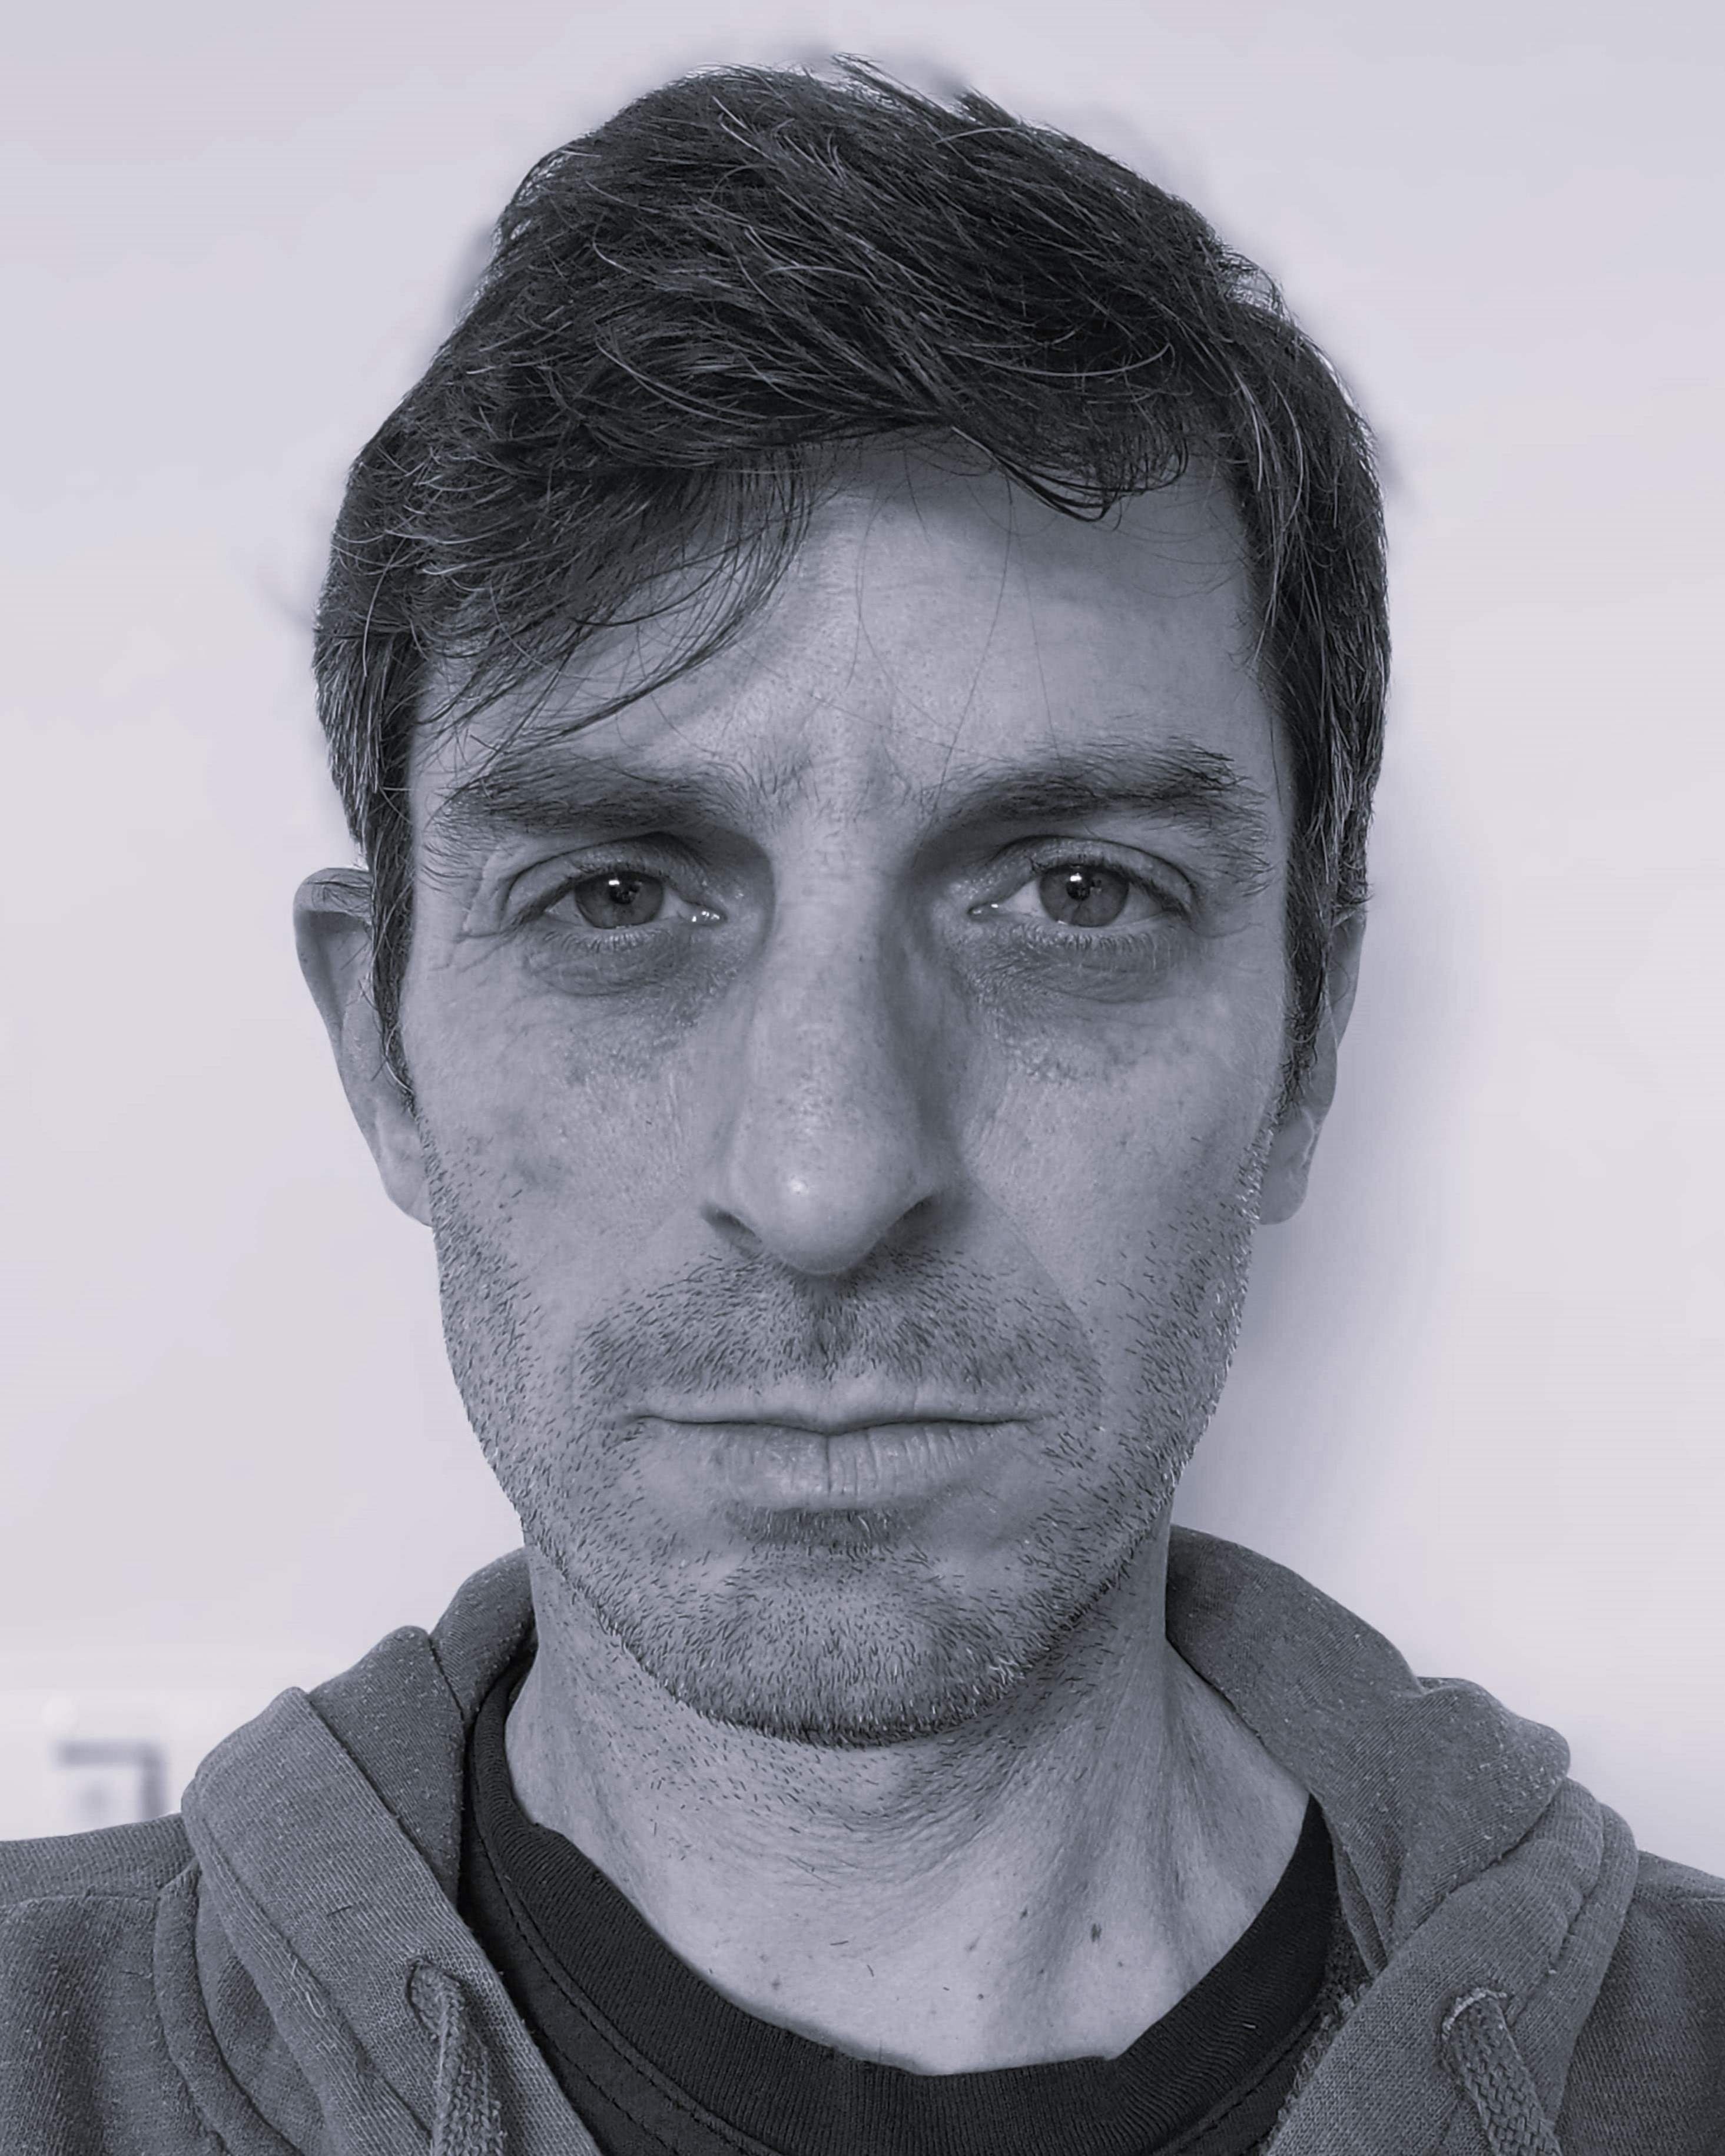
\includegraphics[width=1in,height=1.25in,clip,keepaspectratio]{./Bios/yonatan_shoshan.jpg}}]
    {Yonatan Shoshan} received the B.Sc. degree in electrical and computer engineering from Ben Gurion University, Beer Sheba, Israel, in 2006 and the M.Sc. degree in electrical and computer engineering from University of Calgary, Alberta, Canada, in 2009. He is currently pursuing the Ph.D. degree in electrical and computer engineering at Bar Ilan University, Israel. From 2009 to 2015, he was a digital design engineer in the field of wireless and wired communication with Siverge Networks and Texas Instruments, Israel. His research interests include digital circuits and embedded processing and SoC design, as well as circuits and systems for quantum computers controllers and error correction decoders. 
\end{IEEEbiography}
%</YonatanShoshan>

%<*YehudaRudin>
\begin{IEEEbiography}    [{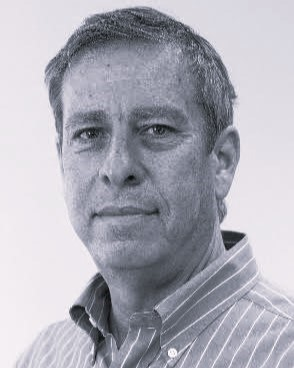
\includegraphics[width=1in,height=1.25in,clip,keepaspectratio]{./Bios/yehuda_rudin.jpg}}]
    {Yehuda Rudin} received the BSc degree in Computer Engineering from the Technion, Haifa, in 1985 and the MSc  degree in Electrical Engineering from Bar-Ilan University, Ramat-Gan, in 2022. He worked at Motorola Semiconductor and later Freescale Semiconductor from 1987 to 2016 in various senior R\&D positions. He became a Freescale Fellow in 2012 and was the General Manager of the Freescale Design Center in Israel from 2013 to 2016. Since 2016, he has been with Bar-Ilan University, where he is a General Manager of the Emerging Nanoscaled Integrated Circuits and Systems (EnICS) Laboratories. Yehuda is currently a Ph.D. student in the Faculty of Engineering, Bar-Ilan University.
\end{IEEEbiography}
%</YehudaRudin>


%<*UdiKra>
\begin{IEEEbiography}    [{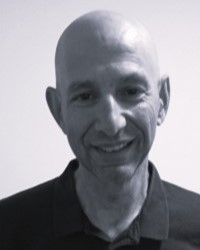
\includegraphics[width=1in,height=1.25in,clip,keepaspectratio]{./Bios/udi_kra.jpg}}]
    {Yehuda (Udi) Kra} received the B.Sc. degree in electrical engineering from the Technion, Israel Institute of Technology in 1985, and the MSc degree from Bar-Ilan University  in 2022. He has over 35 years of experience in design, research, innovation, entrepreneurship, and management in the semiconductor industry, specializing optimized IC solutions.  In 2018  he  joined the Emerging Nanoscaled Integrated Circuits and Systems (EnICS) Research Center at Bar-Ilan University as the Chief Architect of the RISC-V embedded processor project as part of the Israeli Innovation Authority GenPro Consortium. Currently Kra is pursuing his PhD degree focusing on advanced hardware-accelerated Machine-Learning computation platforms.
\end{IEEEbiography}
%</UdiKra>

%%%%%%%%%%%%%%%%%%%%%%%%%%%%%%%%%%%%%%%%%%%%%%%%%%%%
%%%                  UNICAL                      %%%
%%%%%%%%%%%%%%%%%%%%%%%%%%%%%%%%%%%%%%%%%%%%%%%%%%%%
%<*EstebanGarzon>
\begin{IEEEbiography}[{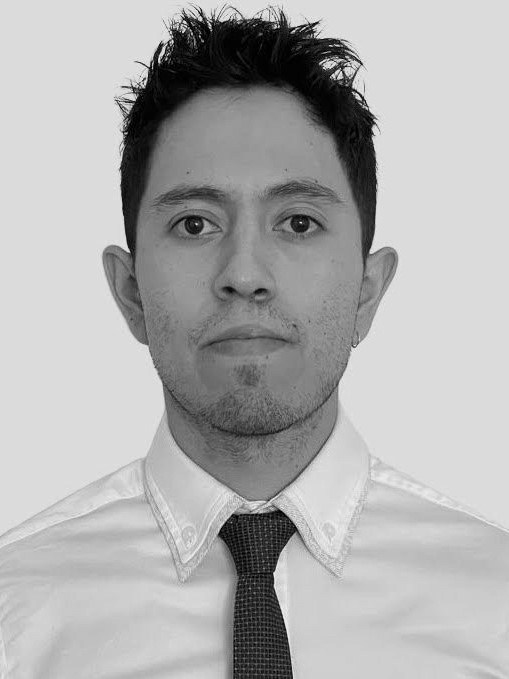
\includegraphics[width=1in,height=1.25in,clip,keepaspectratio]{./Bios/esteban_garzon.jpg}}]{Esteban~Garzón}
    (Member, IEEE) received the Ph.D. degree in electronics engineering from the University of Calabria (UNICAL), Italy, in 2022. He is currently a Postdoctoral Researcher at the Department of Computer Engineering, Modeling, Electronics and Systems Engineering, UNICAL. He has coauthored more than 30 scientific papers in international journals and conferences, and has participated in several IC tapeouts. His research interests include domain-specific hardware accelerators, and electronics/spintronics, cryogenic memories, and standard and emerging technologies for logic, memory, and low-power applications. 
\end{IEEEbiography}
%</EstebanGarzon>

%<*MarcoLanuzza>
\begin{IEEEbiography}[{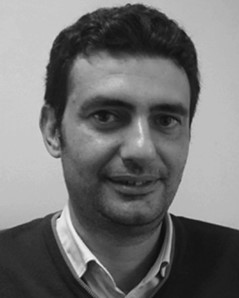
\includegraphics[width=1in,height=1.25in,clip,keepaspectratio]{./Bios/marco_lanuzza.jpg}}]{Marco Lanuzza}
    (Senior Member, IEEE) received the Ph.D. degree in electronic engineering from the Mediterranea University of Reggio Calabria, Reggio Calabria, Italy, in 2005. Since 2006, he has been with the University of Calabria, Rende, Italy, where he is currently an Associate Professor. He has authored over 120 publications in international journals and conference proceedings. His recent research interests include the design of ultralow voltage circuits and systems, the development of efficient models and methodologies for leakage- and variability-aware designs, and the design of digital and analog circuits in emerging technologies. Prof. M. Lanuzza is an Associate Editor of Integration, the VLSI Journal.
\end{IEEEbiography}
%</MarcoLanuzza>


